\solution 
From 
			\eqref{eq:tri-pts},
\begin{align}
    \label{eq:1.1.3,2}
\myvec{
    1 & 1 & 1\\
    \vec{A} & \vec{B} & \vec{C} \\
    } 
    =
    %\label{eq:matthrowoperations}
    \myvec{
    1 & 1 & 1
    \\
    1 & -4 & -3
    \\
    -1 & 6 & -5
    }
     \xleftrightarrow[]{R_3 \leftarrow R_3+R_2}
    \myvec{
    1 & 1 & 1
    \\
    1 & -4 & -3
    \\
    0 & 2 & -8 
    }
    \\
     \xleftrightarrow[]{R_2\leftarrow R_1-R_2}
    \myvec{
    1 & 1 & 1
    \\
    0 & 5 & 4
    \\
    0 & 2 & -8 
    }
     \xleftrightarrow[]{R_3\leftarrow R_3-\frac{2}{5}R_2}
    \myvec{
    1 & 1 & 1
    \\
    0 & 5 & 4
    \\
    0 & 0 & \frac{-48}{5}
    }
\end{align}
There are no zero rows. So,
\begin{align}
    \text{rank}\myvec{
    1 & 1 & 1\\
    \vec{A} & \vec{B} & \vec{C} \\
    } &= 3 
\end{align}  
Hence,  the points $\vec{A},\vec{B},\vec{C}$ are not collinear. 
This is visible in 
\figref{fig1:Triangle}.
\begin{figure}[H]
\centering
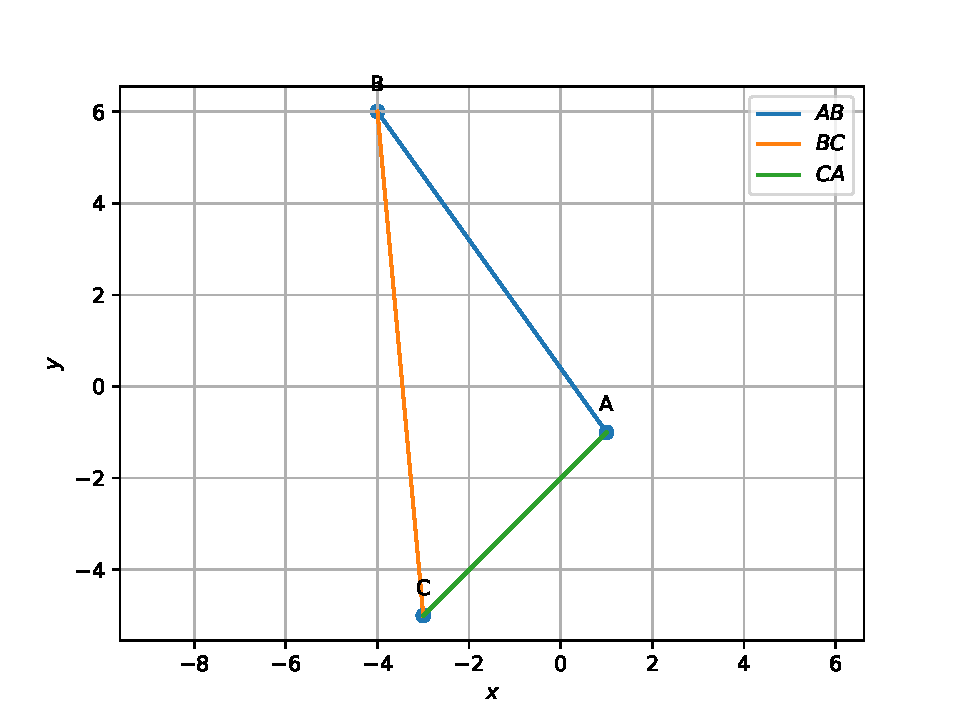
\includegraphics[width=0.75\columnwidth]{figs/triangle/vector.pdf}
\caption{$\triangle ABC$}
\label{fig1:Triangle}
\end{figure}
